%% Preamble %%
%% A minimal LaTeX preamble
%% Some packates are needed to implement
%% Asciidoc features

\documentclass[11pt]{amsart}
\usepackage{geometry}                % See geometry.pdf to learn the layout options. There are lots.
\geometry{letterpaper}               % ... or a4paper or a5paper or ...
%\geometry{landscape}                % Activate for for rotated page geometry
%\usepackage[parfill]{parskip}       % Activate to begin paragraphs with an empty line rather than an indent

\usepackage{tcolorbox}
\usepackage{lipsum}

\usepackage{epstopdf}
\usepackage{color}
% \usepackage[usenames, dvipsnames]{color}
% \usepackage{alltt}


\usepackage{amssymb}
% \usepackage{amsmath}
\usepackage{amsthm}
\usepackage[version=3]{mhchem}


% Needed to properly typeset
% standard unicode characters:
%
\RequirePackage{fix-cm}
\usepackage{fontspec}
\usepackage[Latin,Greek]{ucharclasses}
%
% NOTE: you must also use xelatex
% as the typesetting engine


% \usepackage{fontspec}
% \usepackage{polyglossia}
% \setmainlanguage{en}

\usepackage{hyperref}
\hypersetup{
    colorlinks=true,
    linkcolor=blue,
    filecolor=magenta,
    urlcolor=cyan,
}

\usepackage{graphicx}
\usepackage{wrapfig}
\graphicspath{ {images/} }
\DeclareGraphicsExtensions{.png, .jpg, jpeg, .pdf}

%% \DeclareGraphicsRule{.tif}{png}{.png}{`convert #1 `dirname #1`/`basename #1 .tif`.png}
%% Asciidoc TeX Macros %%


% \pagecolor{black}
%%%%%%%%%%%%


% Needed for Asciidoc

\newcommand{\admonition}[2]{\textbf{#1}: {#2}}
\newcommand{\rolered}[1]{ \textcolor{red}{#1} }
\newcommand{\roleblue}[1]{ \textcolor{blue}{#1} }

\newtheorem{theorem}{Theorem}
\newtheorem{proposition}{Proposition}
\newtheorem{corollary}{Corollary}
\newtheorem{lemma}{Lemma}
\newtheorem{definition}{Definition}
\newtheorem{conjecture}{Conjecture}
\newtheorem{problem}{Problem}
\newtheorem{exercise}{Exercise}
\newtheorem{example}{Example}
\newtheorem{note}{Note}
\newtheorem{joke}{Joke}
\newtheorem{objection}{Objection}





%%%%%%%%%%%%%%%%%%%%%%%%%%%%%%%%%%%%%%%%%%%%%%%%%%%%%%%

%  Extended quote environment with author

\renewenvironment{quotation}
{   \leftskip 4em \begin{em} }
{\end{em}\par }

\def\signed#1{{\leavevmode\unskip\nobreak\hfil\penalty50\hskip2em
  \hbox{}\nobreak\hfil\raise-3pt\hbox{(#1)}%
  \parfillskip=0pt \finalhyphendemerits=0 \endgraf}}


\newsavebox\mybox

\newenvironment{aquote}[1]
  {\savebox\mybox{#1}\begin{quotation}}
  {\signed{\usebox\mybox}\end{quotation}}

\newenvironment{tquote}[1]
  {  {\bf #1} \begin{quotation} \\ }
  { \end{quotation} }

%% BOXES: http://tex.stackexchange.com/questions/83930/what-are-the-different-kinds-of-boxes-in-latex
%% ENVIRONMENTS: https://www.sharelatex.com/learn/Environments

\newenvironment{asciidocbox}
  {\leftskip6em\rightskip6em\par}
  {\par}

\newenvironment{titledasciidocbox}[1]
  {\leftskip6em\rightskip6em\par{\bf #1}\vskip-0.6em\par}
  {\par}



%%%%%%%%%%%%%%%%%%%%%%%%%%%%%%%%%%%%%%%%%%%%%%%%%%%%%%%%

%% http://texblog.org/tag/rightskip/


\newenvironment{preamble}
  {}
  {}

%% http://tex.stackexchange.com/questions/99809/box-or-sidebar-for-additional-text
%%
\newenvironment{sidebar}[1][r]
  {\wrapfigure{#1}{0.5\textwidth}\tcolorbox}
  {\endtcolorbox\endwrapfigure}


%%%%%%%%%%

\newenvironment{comment*}
  {\leftskip6em\rightskip6em\par}
  {\par}

  \newenvironment{remark*}
  {\leftskip6em\rightskip6em\par}
  {\par}


%% Dummy environment for testing:

\newenvironment{foo}
  {\bf Foo.\ }
  {}


\newenvironment{foo*}
  {\bf Foo.\ }
  {}


\newenvironment{click}
  {\bf Click.\ }
  {}

\newenvironment{click*}
  {\bf Click.\ }
  {}


\newenvironment{remark}
  {\bf Remark.\ }
  {}

\newenvironment{capsule}
  {\leftskip10em\par}
  {\par}

%%%%%%%%%%%%%%%%%%%%%%%%%%%%%%%%%%%%%%%%%%%%%%%%%%%%%

%% Style

\parindent0pt
\parskip8pt
%% User Macros %%
%% Front Matter %%

\title{Modeling Examples}
\author{}
\date{}


%% Begin Document %%

\begin{document}
\maketitle
\tableofcontents
\hypertarget{x-\textbf{prepare-your-geometry}}{\section{\textbf{Prepare your geometry}}}
First of all, you need to create the 3D model of your conductor with \texttt{Salome} or \texttt{gmsh} and to make the mesh.
When the mesh is created, with specific names for the volumes and surfaces, export it in \texttt{.med} (example : \texttt{example_mesh.med}) with \texttt{Salome}.
You also need to partition the mesh if you want to do the calculations in parallel, running this command below.


example :


\begin{verbatim}
feelpp_mesh_partitioner --ifile example_mesh.med --part 4 --nochdir
\end{verbatim}

Where \texttt{part} indicate the number of processors you want to use.
This will create a new file, call \texttt{example_mesh_p4.json} that you will use in your configure file.


\hypertarget{x-\textbf{thermoelectric}}{\section{\textbf{ThermoElectric}}}
\hypertarget{x-general-presentation-of-the-files}{\subsection{General presentation of the files}}
You can use ether the linear or the nonlinear model for your calculation, but for our example, we use the linear model, so we select the \texttt{thermoelectric-linear} (respectively \texttt{thermoelectric-nonlinear}) model in the Json file (details in the \hyperlink{code.json}{Example  json}).


When all the files (detailed below) are created, you can run your calculation with this command :


\begin{verbatim}
mpirun -np "number_of_processor_you_have_chosen_in_the_partition" feelpp_hfm_thermoelectric_model_3D_V1T1_N1 --config-file "name_of_your_file.cfg"
\end{verbatim}

\hypertarget{x-material}{\subsubsection{Material}}
\begin{center}
\begin{tabular}{|c|c|}
\hline
$\alpha$ & alpha \\ 
$\sigma_{0}$ / $\sigma$ & sigma0 / sigma \\ 
k${}_{0}$ / k & k0 / k \\ 
T${}_{0}$ & T0 \\ 
\hline
\end{tabular}
\end{center}

There is a dedicated section in the Json file, named \texttt{Materials}, to configure the magnet properties.
The structure of a json file is as follows (conditions are details in \hyperlink{x-condition}{Condition}) :


\begin{verbatim}
{
    "Name": "ThermoElectric",
    "ShortName":"TE",
    "Model":"thermoelectric-linear",
    "Materials":
    {
	   "Name_of_the_first_volume":
	    {
	     "name":"material_of_this_volume",
	      "alpha":"_",
	      "T0":"_",
	      "sigma0":"_",
	      "k0":"_",
	      "sigma":"sigma0/(1+alpha*(T-T0)):sigma0:alpha:T:T0",
	      "k":"k0*T/((1+alpha*(T-T0))*T0):k0:T:alpha:T0"
	    },
	  "other_volume":
	   {
	    ...
	   }
  },
    "BoundaryConditions":
    {
	   "first_condition(like potential or temperature)":
	    {
	     "type_of_condition":
	      {
		      "Surface_concerned_by_the_condition":
		        {
		          "expr1":"_",
		          "expr2":"_"
		        },
		      "Surface_concerned_by_the_condition":
		        {
		          "expr1":"_",
		          "expr2":"_"
		        }
	      }
	   },
	    "other_condition":
	     {
	      ...
	     }
    },
    "PostProcess":
      {
	     "Fields":["temperature","potential","current"]
      }
}
\end{verbatim}

\admonition{WARNING}{The name of the volumes and surfaces must be the same as defined in \texttt{Salome}.
Be careful to the units of the material properties. They need to be consistent with the length unit used for the rest.
For instance the length unit is in \textbf{mm} in \hyperlink{test.json}{quarter-turn3Djson}.}
It is also necessary to create a file to configure the calculation, call \texttt{.cfg} file (example \hyperlink{example-file.cfg}{thermoelectric_3D_V1T1_N1_cvgcfg (for the T1V1 model)}).
It will configure which file you will use in your calculations and which type of solver you use (here we use the Krylov method to solve both \texttt{electro} and \texttt{thermal} problem).


\begin{verbatim}
dim=3
geofile="name_of_the_file_created_by_the_partition.json" (or .msh)
geofile-path=$cfgdir


conductor_volume="name_of_your_volume"

[thermoelectric]
model_json=$cfgdir/"name_of_your_file.json"
weakdir=false

[electro]
pc-type=gamg
#ksp-monitor=true
ksp-rtol="relative_convergence_tolerance"
ksp-atol="absolute_convergence_tolerance"
ksp-maxit="maximum_number_of_iterations"
ksp-use-initial-guess-nonzero=1

[thermal]
pc-type=gamg
#ksp-monitor=true
ksp-rtol="relative_convergence_tolerance"
ksp-atol="absolute_convergence_tolerance"
ksp-use-initial-guess-nonzero=1
\end{verbatim}

There are few differences between the linear and the nonlinear calculation.
For the nonlinear model, just add this lines in the section \texttt{thermoelectric} :


{\bf nonlinear}\vspace{-1\baselineskip}
\begin{verbatim}
eps_potential=1.e-4
eps_temperature=1.e-4
resolution=picard
itmax_picard=10
update_intensity=true
marker_intensity="the_surface"
target_intensity="the_intensity" (be careful of the sign)
eps_intensity=1.e-2
verbosity=2
\end{verbatim}

We can define the current I using the Ohm’s law, defining the voltage ine the \texttt{json} file.


\hypertarget{x-condition}{\subsubsection{Condition}}
There are three type of conditions :


1 \textbf{Dirichlet}


\begin{verbatim}
"Dirichlet": //values of the solution known at the limits of the domain
  {
    "Surface":
      {
        "expr1":"Value_of_the_solution"
        "expr2":"Volume_concerned"
      },
    "other_surface":
      {
        "expr1":"Value_of_the_solution"
        "expr2":"Volume_concerned"
      }
  }
\end{verbatim}

2 \textbf{Neumann}


\begin{verbatim}
"Neumann":  // value of the derivative of the solution knowns at the limit of the domain
  {
    "Surface":
      {
        "expr":"Value_of_derivatives_of_the_solution"
      },
    "other_surface":
      {
        "expr":"Value_of_derivatives_of_the_solution"
      }
  }
\end{verbatim}

3 \textbf{Robin}


\begin{verbatim}
"Robin":   // linear relation between the value and the derivative at the limits of the domain
  {
    "Surface":
      {
        "expr1":"Value_of_derivatives_of_the_solution"
        "expr2":"Value_of_the_solution"
      },
    "other_surface":
      {
        "expr1":"Value_of_derivatives_of_the_solution"
        "expr2":"Value_of_the_solution"
      }
  }
\end{verbatim}

\admonition{WARNING}{Your have to set a condition for each surfaces you have defined.
For those where there is no conditions, set an homogeneous Neumann condition (\texttt{"expr":"0"})}
\hypertarget{x-examples}{\subsection{Examples}}
\hypertarget{x-current-sensor}{\subsubsection{Current sensor}}
Here we want to model a current sensor placed in the connection of a magnet.
This sensor consist in 6 constantan plates placed between the connectors as shown in the images.
The goal is to allow the users to directly see the evolution of the current by measuring the potential in the connection.
The main problem is the temperature reached by the sensor, due to the high current, the fusion of the constantan being around 1500 K, but we don’t want to exceed an elevation of 200 degree.
Because an excessive increase of the temperature will
We model all of this with \texttt{salome} and do the mesh.
The mesh is more precise on the sensor (the 6 constantan plates)


\begin{wrapfigure}{l}{4.75truein}
\centering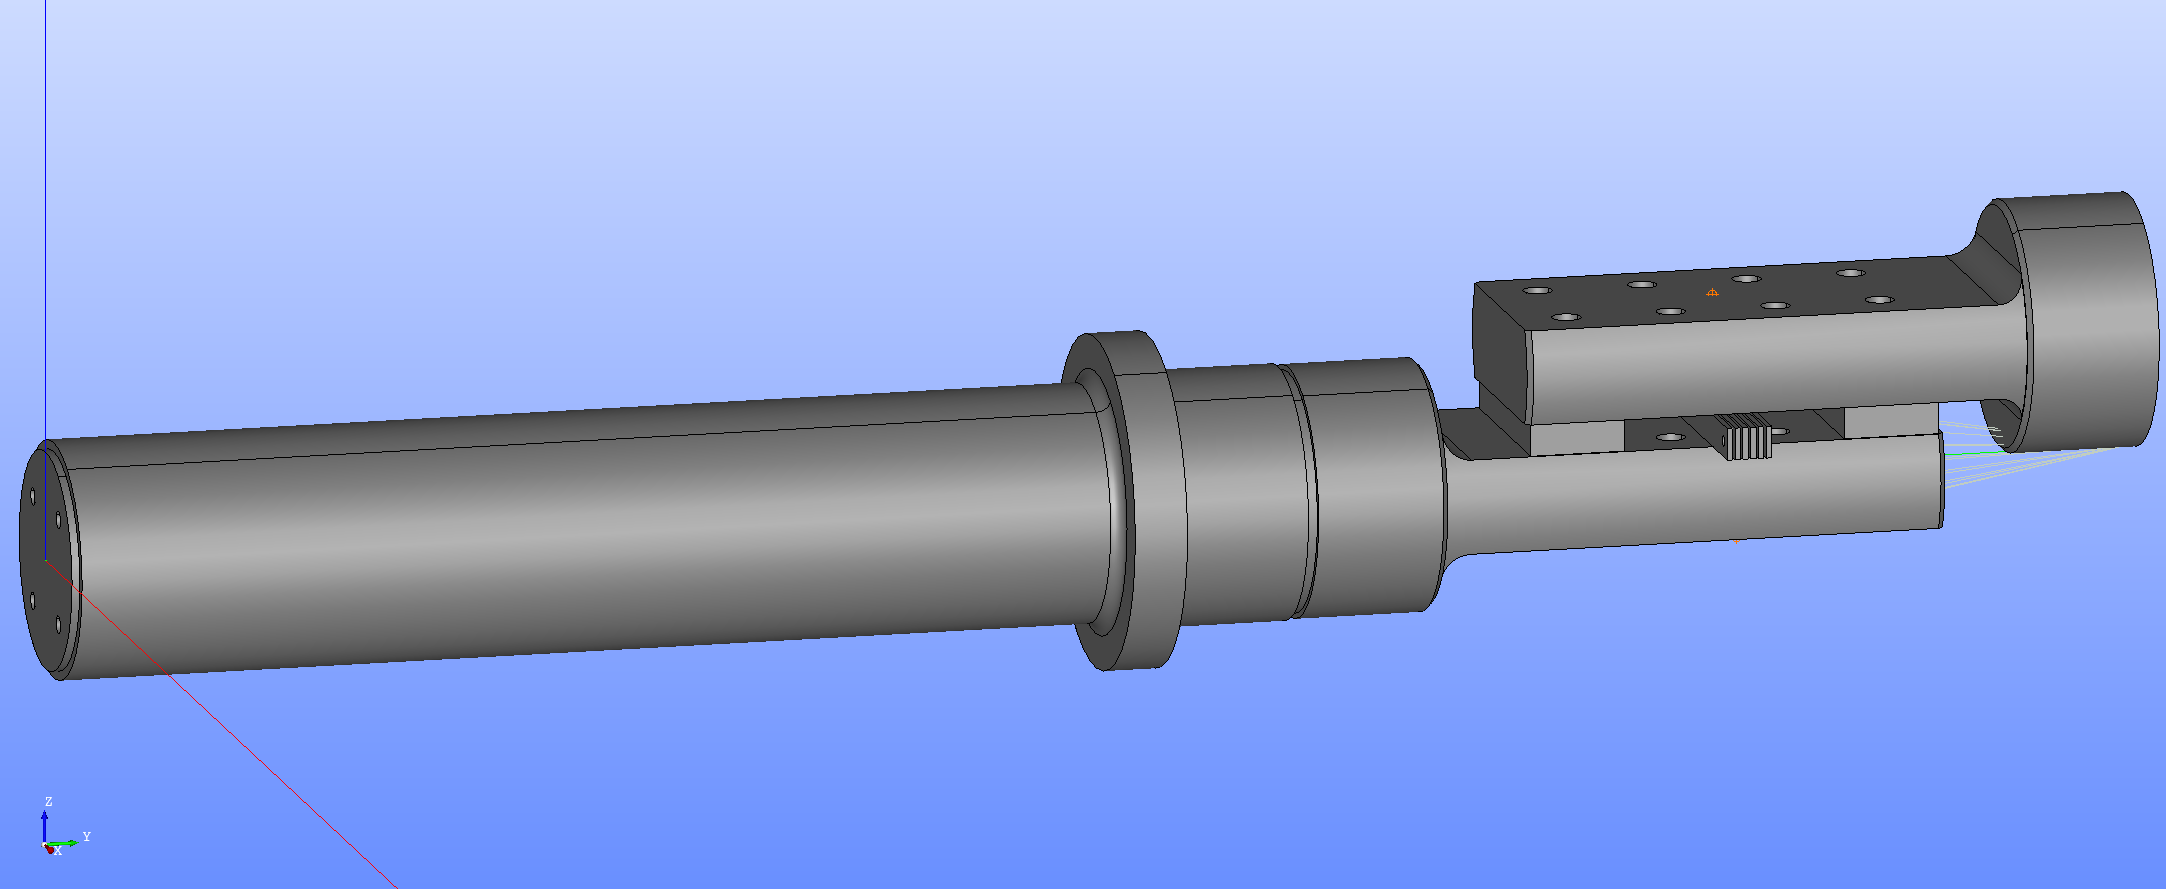
\includegraphics[width=4.75truein]{./images/learning/thermoelectric/Ensemble_CapteurCourant.png}


\end{wrapfigure}

\begin{wrapfigure}{r}{4.75truein}
\centering\includegraphics[width=4.75truein]{./images/learning/thermoelectric/capteurcourant.png}


\end{wrapfigure}

\hypertarget{x-parameters}{\paragraph{Parameters}}
There are 8 volumes, 2 connectors in copper and the 6 constantan plates which constitute the sensor.


\begin{verbatim}
{
    "Name": "ThermoElectric",
    "ShortName":"TE",
    "Model":"thermoelectric-linear",
    "Materials":
    {
	"A1":
	{
	    "name":"A1",
	    "alpha":"3.35e-3",
	    "T0":"293",
	    "sigma0":"58e+3",
	    "k0":"0.38",
	    "sigma":"sigma0/(1+alpha*(T-T0)):sigma0:alpha:T:T0",
	    "k":"k0*T/((1+alpha*(T-T0))*T0):k0:T:alpha:T0"
	},
	"CurrentLead_1":
	{
	    "name":"CurrentLead_1",
	    "alpha":"3.35e-3",
	    "T0":"293",
	    "sigma0":"58e+3",
	    "k0":"0.38",
	    "sigma":"sigma0/(1+alpha*(T-T0)):sigma0:alpha:T:T0",
	    "k":"k0*T/((1+alpha*(T-T0))*T0):k0:T:alpha:T0"
	},
	"Constantan_1":
	{
	    "name":"Constantan_1",
	    "alpha":"0",
	    "T0":"293",
	    "sigma0":"2.04e+3",
	    "k0":"0.019",
	    "sigma":"sigma0/(1+alpha*(T-T0)):sigma0:alpha:T:T0",
	    "k":"k0*T/((1+alpha*(T-T0))*T0):k0:T:alpha:T0"
	},
	"Constantan_2":
	{
	    "name":"Constantan_2",
	    "alpha":"0",
	    "T0":"293",
	    "sigma0":"2.04e+3",
	    "k0":"0.019",
	    "sigma":"sigma0/(1+alpha*(T-T0)):sigma0:alpha:T:T0",
	    "k":"k0*T/((1+alpha*(T-T0))*T0):k0:T:alpha:T0"
	},
	"Constantan_3":
	{
	    "name":"Constantan_3",
	    "alpha":"0",
	    "T0":"293",
	    "sigma0":"2.04e+3",
	    "k0":"0.019",
	    "sigma":"sigma0/(1+alpha*(T-T0)):sigma0:alpha:T:T0",
	    "k":"k0*T/((1+alpha*(T-T0))*T0):k0:T:alpha:T0"
	},
	"Constantan_4":
	{
	    "name":"Constantan_4",
	    "alpha":"0",
	    "T0":"293",
	    "sigma0":"2.04e+3",
	    "k0":"0.019",
	    "sigma":"sigma0/(1+alpha*(T-T0)):sigma0:alpha:T:T0",
	    "k":"k0*T/((1+alpha*(T-T0))*T0):k0:T:alpha:T0"
	},
	"Constantan_5":
	{
	    "name":"Constantan_5",
	    "alpha":"0",
	    "T0":"293",
	    "sigma0":"2.04e+3",
	    "k0":"0.019",
	    "sigma":"sigma0/(1+alpha*(T-T0)):sigma0:alpha:T:T0",
	    "k":"k0*T/((1+alpha*(T-T0))*T0):k0:T:alpha:T0"
	},
	"Constantan_6":
	{
	    "name":"Constantan_6",
	    "alpha":"0",
	    "T0":"293",
	    "sigma0":"2.04e+3",
	    "k0":"0.019",
	    "sigma":"sigma0/(1+alpha*(T-T0)):sigma0:alpha:T:T0",
	    "k":"k0*T/((1+alpha*(T-T0))*T0):k0:T:alpha:T0"
	}
},
\end{verbatim}

\hypertarget{x-conditions}{\paragraph{Conditions}}
\begin{verbatim}
"BoundaryConditions":
{
"potential":
{
  "Dirichlet":
  {
"V0":
{
    "expr1":"0",
    "expr2":"A1"
},
"V1":
{
    "expr1":"0.1",
    "expr2":"CurrentLead_1"
}
  }
},
"temperature":
{
  "Dirichlet":
  {
"V0":
{
    "expr1":"293",
    "expr2":"A1"
},
"V1":
{
    "expr1":"293",
    "expr2":"CurrentLead_1"
}
  }
}
},
"PostProcess":
{
"Fields":["temperature","potential","current"]
}
}
\end{verbatim}

There is also a specific file to study only one plate, to be more precise on the temperature reach.
We can use here a nonlinear model for the thermoelectric study.


\begin{verbatim}
{
    "Name": "ThermoElectric",
    "ShortName":"TE",
    "Model":"thermoelectric-nonlinear",
    "Materials":
    {
	"Constantan_1":
	{
	    "name":"Constantan_1",
	    "alpha":"2.e-5",
	    "T0":"293",
	    "sigma0":"2.04e+3",
	    "k0":"19.5e-3",
	    "sigma":"sigma0/(1+alpha*(T-T0)):sigma0:alpha:T:T0",
	    "k":"k0*T/((1+alpha*(T-T0))*T0):k0:T:alpha:T0"
	}
    },
    "BoundaryConditions":
    {
	"potential":
	{
	    "Dirichlet":
	    {
		"Interface_0":
		{
		    "expr1":"0",
		    "expr2":"Constantan_1"
		},
		"Interface_1":
		{
		    "expr1":"0.1153",
		    "expr2":"Constantan_1"
		}
	    },
	    "Neumann":
	    {
		"Fixer":
		{
		    "expr":"0"
		},
		"Free_edge":
		{
		    "expr":"0"
		}
	    }
	},
	"temperature":
	{
	    "Robin":
	    {
		"Free_edge":
		{
		    "expr1":"50.e-6",  //the heat transfer coefficient
		    "expr2":"293"
		}
	    },
	    "Neumann":
	    {
		"Fixer":
		{
		    "expr":"0"
		},
		"Interface_0":
		{
		    "expr":"0"
		},
		"Interface_1":
		{
		    "expr":"0"
		}
	    }
	}
    },
    "PostProcess":
    {
	"Fields":["temperature","potential","current","joules"]
    }
}
\end{verbatim}

\hypertarget{x-results}{\paragraph{Results}}
First we can see the potential we should be measuring.


\begin{figure}[h]{}
\centering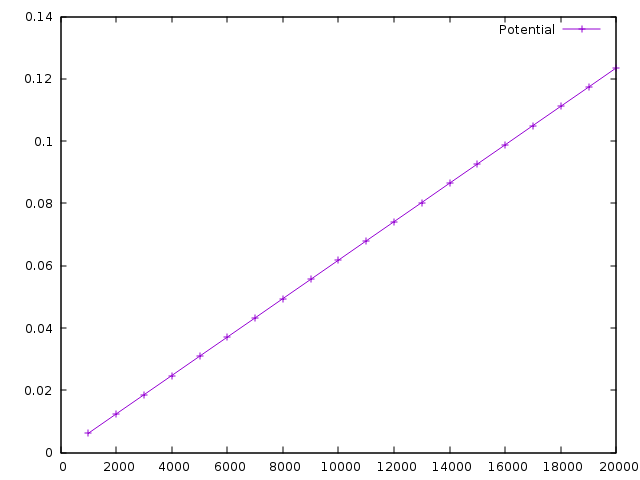
\includegraphics[width=6.0truein]{./images/learning/thermoelectric/Potential.png}
\caption{Potential as a function of current}
\centering
\end{figure}

Therefore, we need a voltmeter which can be precise between 0.01 and 0.15 Volt.


Next, we want to control the temperature reached by the sensor, the purpose being not to destroy the sensor.
The melting temperature of the Constantan is near 1500 K, but we want to stop well before reaching this point to avoid deformations of the sensor.
The main parameter that we can control is the heat transfer coefficient \textbf{h} ($W.m^{-2} .K^{-1}$).
This coefficient \textbf{h} can be control by displaying or not a ventilator to be in natural or forced convection.


\begin{figure}[h]{}
\centering\includegraphics[width=9.0truein]{./images/learning/thermoelectric/Temperature_Max.png}
\caption{Temperature max in 1 plate as a function of current}
\centering
\end{figure}

Here we see that in natural convection (h=15), the temperature reached is by far too high.


\begin{figure}[h]{}
\centering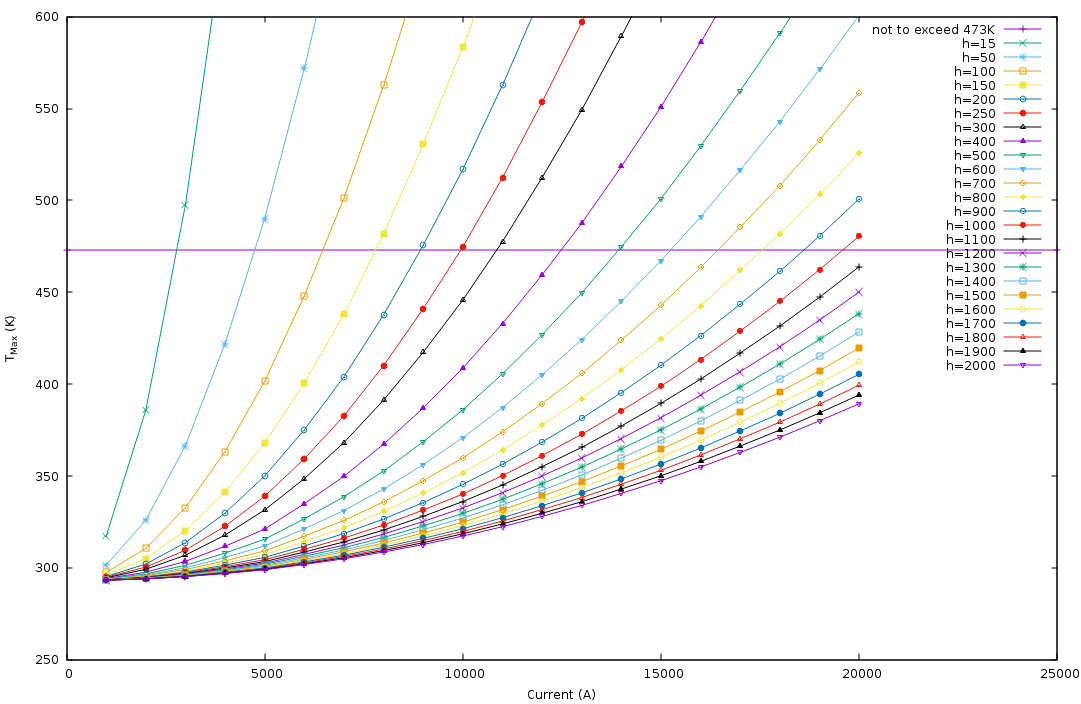
\includegraphics[width=9.0truein]{./images/learning/thermoelectric/Temperature_Max_Zoom2.png}
\caption{Temperature max in 1 plate as a function of current, forced convection only}
\centering
\end{figure}

A heat transfer coefficient maximum allow to set a higher current but is more difficult to set up.


\hypertarget{x-double-helix}{\subsubsection{Double Helix}}
For this piece, the purpose is to see the elevation of the temperature in the conductor around the double helix.
We model a double helix on \texttt{salome} then do the mesh.


\begin{figure}[h]{}
\centering\includegraphics[width=5.0truein]{./images/learning/thermoelectric/Double_Helix_Geometry.png}
\caption{Double Helix on `Paraview`}
\centering
\end{figure}

\hypertarget{x-parameters}{\paragraph{Parameters}}
\begin{verbatim}
{
    "Name": "ThermoElectric",
    "ShortName": "TE",
    "Model":"thermoelectric-nonlinear",
    "Materials":
    {
	"Cu":
	{
	    "name":"copper",
	    "alpha":"3.75e-3",
	    "T0":"293",
	    "sigma0":"56.e+3",
	    "k0":"0.4",
	    "sigma":"sigma0/(1+alpha*(T-T0)):sigma0:alpha:T:T0",
	    "k":"k0*T/((1+alpha*(T-T0))*T0):k0:T:alpha:T0"
	},
	"Glue0":
	{
	    "name":"glue0",
	    "alpha":"0",
	    "T0":"293",
	    "sigma0":"0",
	    "k0":"1.2e-3",
	    "sigma":"sigma0/(1+alpha*(T-T0)):sigma0:alpha:T:T0",
	    "k":"k0*T/((1+alpha*(T-T0))*T0):k0:T:alpha:T0"
	},
	"Glue1":
	{
	    "name":"glue1",
	    "alpha":"0",
	    "T0":"293",
	    "sigma0":"0",
	    "k0":"1.2e-3",
	    "sigma":"sigma0/(1+alpha*(T-T0)):sigma0:alpha:T:T0",
	    "k":"k0*T/((1+alpha*(T-T0))*T0):k0:T:alpha:T0"
	}
    },
\end{verbatim}

\hypertarget{x-conditions}{\paragraph{Conditions}}
\begin{verbatim}
"BoundaryConditions":
{
"potential":
{
  "Dirichlet":
  {
"V1":
{
    "expr1":"9",
    "expr2":"Cu"
},
"V0":
{
    "expr1":"0",
    "expr2":"Cu"
}
  },
  "Neumann":
  {
"Interface0_1":
{
    "expr":"0"
},
"Interface0_2":
{
    "expr":"0"
},
"Rint":
{
    "expr":"0"
},
"Rext":
{
    "expr":"0"
},
"iRint1":
{
    "expr":"0"
},
"iRext1":
{
    "expr":"0"
},
"iRint2":
{
    "expr":"0"
},
"iRext2":
{
    "expr":"0"
}
  }
},
"temperature":
{
  "Robin":
  {
"Rint":
{
    "expr1":"85000.e-6",
    "expr2":"293"
},
"Rext":
{
    "expr1":"85000.e-6",
    "expr2":"293"
},
"iRint1":
{
    "expr1":"85000.e-6",
    "expr2":"293"
},
"iRext1":
{
    "expr1":"85000.e-6",
    "expr2":"293"
},
"iRint2":
{
    "expr1":"85000.e-6",
    "expr2":"293"
},
"iRext2":
{
    "expr1":"85000.e-6",
    "expr2":"293"
}
  },
  "Neumann":
  {
"Interface0_1":
{
    "expr":"0"
},
"Interface0_2":
{
    "expr":"0"
},
"V0":
{
    "expr":"0"
},
"V1":
{
    "expr":"0"
}
  }
}
},
"PostProcess":
{
"Fields":["temperature","potential","current"]
}
}
\end{verbatim}

\hypertarget{x-results}{\paragraph{Results}}
We can see the repartition of the temperature in the helix.


\begin{figure}[h]{}
\centering\includegraphics[width=9.0truein]{./images/learning/thermoelectric/Double_Helix_temperature.png}
\caption{Temperature's repartition on paraview}
\centering
\end{figure}

We can note that the peak temperature is inside the double helix.


\hypertarget{x-validity}{\subsection{Validity}}
In this example, we approximate the magnet with an axisymmetric copper torus.Thus we can consider only a quarter of this torus for our study.
The torus is modeled thanks to the file geo, which also name the volume (\texttt{omega}) and each surface.


\begin{figure}[h]{}
\centering\includegraphics[width=3.0truein]{./images/learning/thermoelectric/quarter-turn3D.png}
\caption{Model of the quarter of torus on `Gmsh`}
\centering
\end{figure}

\hypertarget{x-equations}{\paragraph{Equations}}
First of all, we start with the standard heat equation, with the heat from the Joule effect :

\[
\rho C_{p}\frac{\partial T}{\partial t} - \nabla.(k \nabla T)=\sigma(\frac{U}{2\pi r})^{2}
\]



Coefficients $\sigma$ and k are in fact, temperature-dependent, shown in this equations :


\begin{itemize}

\item $\sigma=\frac{\sigma_ {0}}{1 + \alpha(T-T_{ref})}$

\item $k=k_{0}\frac{T}{(1+\alpha(T-T_{ref}))T_{ref}}$

\end{itemize}


But, for the next, we consider that $\alpha=0$ and T=T${}_{ref}$.
Thereby, we are in a linear problem that we can solve with the \texttt{thermoelectric-linear} model in the Json file.


In our case, we consider that T only depends on the radius, so $\frac{\partial T}{\partial t}=0$.
We can now consider this equation :

\[
T=A\log(r)-\frac{\sigma}{2k}(\frac{U}{2\pi})^{2} \log^{2}(r)+B
\]



The constants A and B are determined by the boundary conditions (Dirichlet and Robin).


Finally, we have this equation :

\[
T=-a \log(\frac{r}{r_{0}})^{2} + T_{max}
\]



\begin{itemize}

\item $T_{max}=\frac{2ak}{h_{1}r_{1}+h_{2}r_{2}}\log(\frac{r_{2}}{r_{1}})+\frac{h_{1}r_{1}T_{w1}+h_{2}r_{2}T_{w2}}{h_{1}r_{1}+h_{2}r_{2}}+ a\frac{h_{1}r_{1}log(\frac{r_{1}}{r_{0}})^{2} +h_{2}r_{2}log(\frac{r_{2}}{r_{0}})^{2}}{h_{1}r_{1}+h_{2}r_{2}}$

\item $r_{0}=e^{\frac{\frac{T_{w2}-T_{w1}}{b}+\frac{ac}{b}}{2a}}$

\item $a=\frac{\sigma_{0}}{2k}(\frac{U}{2\pi})^{2}$

\item $b=k(\frac{1}{h_{1}r_{1}}+\frac{1}{h_{2}r_{2}})+\log(\frac{r_{2}}{r_{1}})$

\item $c=\log(\frac{r_{2}}{r_{1}})\log(r_{1}r_{2}) + 2k (\frac{\log(r_{1})}{h_{1}r_{1}}+\frac{\log(r_{2})}{h_{2}r_{2}})$

\end{itemize}


r${}_{0}$ is the radius for which the temperature is at its maximum.


\hypertarget{x-parameters}{\paragraph{Parameters}}
In our case, we choose the parameters like this :


\begin{center}
\begin{tabular}{|c|c|c|c|c|}
\hline
$\sigma_{0}$ & electrical conductivity at T${}_{0}$ & $[52.10^{6}; 58.10^{6}$] & $58.10^{6}$ & $S.m^{-1}$ \\ 
k & thermal conductivity & [360;380] & 380 & $W.m^{-1} .K^{-1}$ \\ 
r${}_{1}$ & internal radius & $1.10^{-3}$ & $1.10^{-3}$ & m \\ 
r${}_{2}$ & internal radius & $2.10^{-3}$ & $2.10^{-3}$ & m \\ 
T${}_{w1}$ & water cooling temperature on radius r${}_{1}$ & [293;310] & 293 & K \\ 
T${}_{w2}$ & water cooling temperature on radius r${}_{2}$ & [293;310] & 293 & K \\ 
h${}_{2}$ & heat transfer coefficient & [70000;90000] & 80000 & $W.m^{-2} .K^{-1}$ \\ 
h${}_{1}$ & heat transfer coefficient & $h_{1}=h_{2}\frac{r_{2}}{r_{1}}$ & $W.m^{-2} .K^{-1}$ \\ 
V${}_{0}$ & electrical potential & - & 0.3 & V \\ 
\hline
\end{tabular}
\end{center}

\hypertarget{x-conditions}{\paragraph{Conditions}}
We set 2 conditions :


\begin{itemize}

\item Dirichlet for the potential : V${}_{in}$=0 V  and  $V_{out}=V_{0}\frac{1}{4}=0.075  V$ \emph{because we consider only one quarter of the torus}.

\item Robin for the temperature :

\begin{itemize}

\item On r${}_{int}$ : $h_{1}=80000\frac{r_{2}}{r_{1}}=160000 W.m^{-2} .K^{-1}$  and  T${}_{w1}$=293 K

\item On r${}_{ext}$ : h${}_{2}$=80000 $W.m^{-2} .K^{-1}$  and  T${}_{w2}$= 293 K

\end{itemize}

\end{itemize}


\hypertarget{x-results}{\paragraph{Results}}
\begin{wrapfigure}{l}{5.0truein}
\centering\includegraphics[width=5.0truein]{./images/learning/thermoelectric/Temperature_paraview.png}


\end{wrapfigure}

\begin{wrapfigure}{r}{4.5truein}
\centering\includegraphics[width=4.5truein]{./images/learning/thermoelectric/TemperatureTH.png}


\end{wrapfigure}

We can vary the degree of the finite element from 1 (linear) to 2 (quadratic). \\
To prove the convergence towards the theory, we plot the difference between L${}_{2}$/H${}_{1}$ and the theoretical formulas for T and V.
The scale is logarithmic, to see directly the slope and note that it is directly linked to the degree of the finite element used.



\[
T=-a \log(\frac{r}{r_{0}})^{2} + T_{max}
\]




\[
V=\frac{0.3*atan2(x,y)}{2\pi}
\]



\begin{itemize}

\item For L2, we have directly the output on the table obtained whether for T or for V

\item For H1, we need to do a quadratical mean between the H1 and L2 of the table ($\sqrt{H1^{2} +L2^{2}}$) for T and V

\end{itemize}


\begin{wrapfigure}{l}{4.75truein}
\centering\includegraphics[width=4.75truein]{./images/learning/thermoelectric/L2V.png}


\end{wrapfigure}

\begin{wrapfigure}{r}{4.75truein}
\centering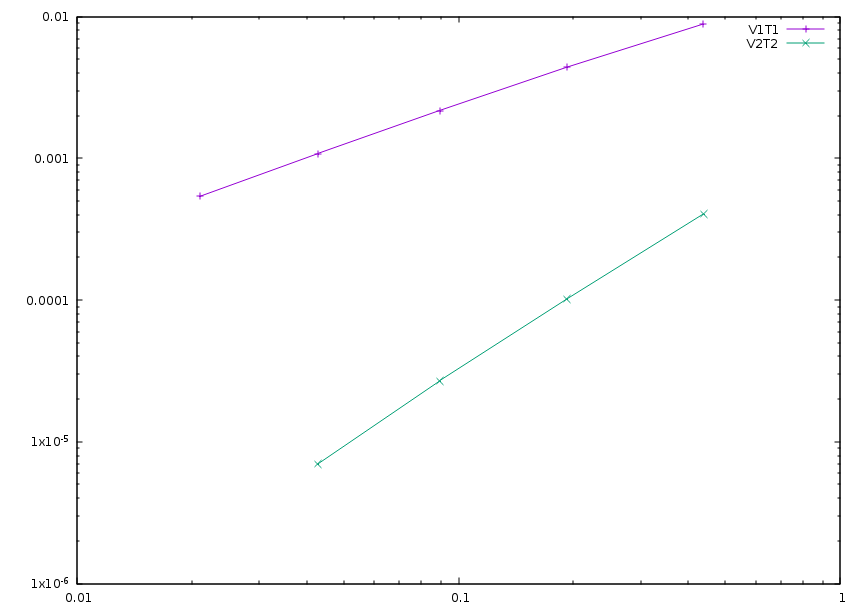
\includegraphics[width=4.75truein]{./images/learning/thermoelectric/H1V.png}


\end{wrapfigure}

\begin{wrapfigure}{l}{4.75truein}
\centering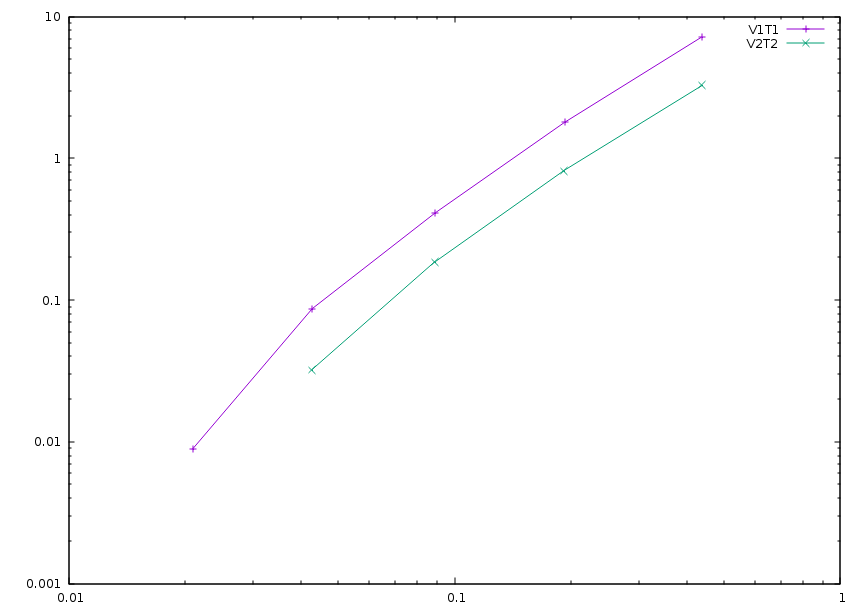
\includegraphics[width=4.75truein]{./images/learning/thermoelectric/L2T.png}


\end{wrapfigure}

\begin{wrapfigure}{r}{4.75truein}
\centering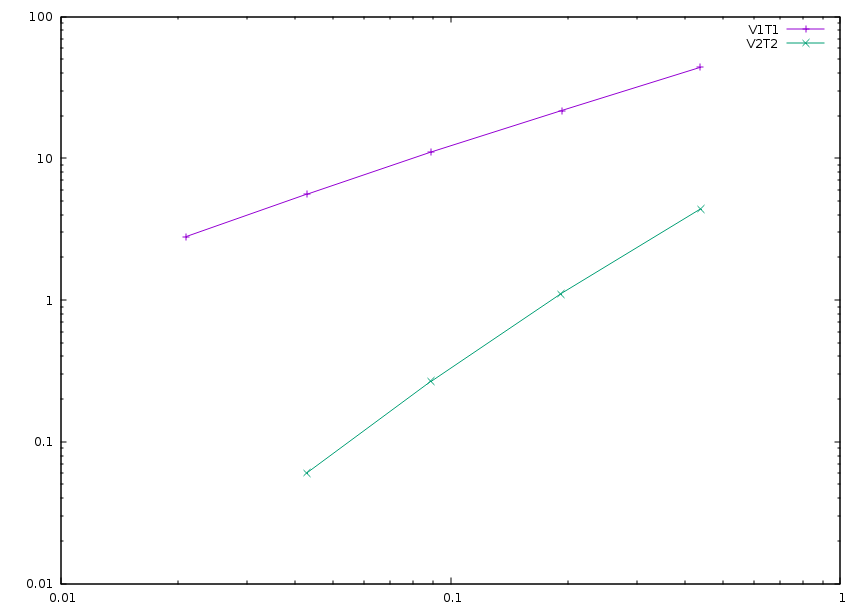
\includegraphics[width=4.75truein]{./images/learning/thermoelectric/H1T.png}


\end{wrapfigure}

\hypertarget{x-code}{\paragraph{Code}}
For the modelisation of the quarter of torus, we create the geometry and the mesh on \texttt{Salome} and export the file in \texttt{.geo}


\begin{verbatim}
// Define Main params
Unit = 1.e-3;
lc = 1*Unit;
lc_ext = 3*lc;
lc_inf = 1*lc;

h=0.2;
r1=1;
r2=2;
L=2*r2;



Mesh.ElementOrder = 1;
Point(1) = {0, 0, -L, h};
Point(2) = {r1, 0, -L, h};
Point(3) = {r2, 0, -L, h};
Point(4) = {0, r1, -L, h};
Point(5) = {0, r2, -L, h};
Circle(1) = {2, 1, 4};
Circle(2) = {3, 1, 5};
Line(3) = {4, 5};
Line(4) = {2, 3};
Line Loop(5) = {3, -2, -4, 1};
Plane Surface(1) = {5};

out[] = Extrude {0,0,L} {Surface{1};};

Physical Volume("omega") = {out[1]};
Physical Surface("top") = {out[0]};
Physical Surface("bottom") = {1};
Physical Surface("Rint") = {out[5]};
Physical Surface("Rext") = {out[3]};
Physical Surface("in") = {out[2]};
Physical Surface("out") = {out[4]};
\end{verbatim}

Next step is to create a file.json which define the model we will use, the material and sets the conditions.


\begin{verbatim}
{
    "Name": "ThermoElectric",
    "ShortName":"TE",
    "Model":"thermoelectric-linear",

    "Materials":
    {
        "omega":
        {
            "name":"copper",
            "alpha":"3.35e-3",
            "T0":"293",
            "sigma0":"58e+3",
            "k0":"0.38",
            "sigma":"sigma0/(1+alpha*(T-T0)):sigma0:alpha:T:T0",
            "k":"k0*T/((1+alpha*(T-T0))*T0):k0:T:alpha:T0"
        }
    },
    "BoundaryConditions":
    {
        "potential":
        {
            "Dirichlet":
            {
                "in":
                {
                    "expr1":"0",
		    "expr2":"omega"
                },
                "out":
                {
                    "expr1":"0.3/4.", // since we consider only 1/4th of a torus
		    "expr2":"omega"
                }
        },
        "temperature":
        {
            "Robin":
            {
                "Rext":
                {
                    "expr1":"0.08",
                    "expr2":"293"
                },
                "Rint":
                {
                    "expr1":"0.08*(2./1.)",
                    "expr2":"293"
                }
            }
        }
    },
    "PostProcess":
    {
        "Fields":["temperature","potential","current"]
    }
}
\end{verbatim}

Lastly, we create a file.cfg to configure what we will calculate.


{\bf \hypertarget{example-file.cfg}{thermoelectric_3D_V1T1_N1_cvg.cfg (for the T1V1 model)}}\vspace{-1\baselineskip}
\begin{verbatim}
dim=3
geofile=quarter-turn3D.geo
geofile-path=$cfgdir
gmsh.hsize=0.2

conductor_volume=omega

[convergence]
max_iter=5

[functions]
#V_exact
f=0.3*atan2(x,y)/(2*pi):x:y:z
#T_exact
g=600.312-58.e+3/(2*0.38)*(0.3/(2*pi))^2*log(sqrt(x*x+y*y)/sqrt(1*2))^2:x:y:z

[thermoelectric]
model_json=$cfgdir/quarter-turn3D.json
weakdir=false

[electro]
pc-type=gamg
#ksp-monitor=true
ksp-rtol=1e-7
ksp-atol=1e-5
ksp-maxit=2000
ksp-use-initial-guess-nonzero=1

[thermal]
pc-type=gamg
#ksp-monitor=true
ksp-rtol=1e-8
ksp-atol=1e-6
ksp-use-initial-guess-nonzero=1
\end{verbatim}

Finally, to execute our program, run this command :


{\bf to study the convergence}\vspace{-1\baselineskip}
\begin{verbatim}
mpirun -np 4 feelpp_test_convergence_3D_V1T1_N1  --config-file thermoelectric_3D_V1T1_N1_cvg.cfg
\end{verbatim}

It will create a table with all the informations you need. For our example, we showed the convergence using L2 and H1 (in section \hyperlink{x-results}{Results}).


{\bf to apply for a real case (theory not known)}\vspace{-1\baselineskip}
\begin{verbatim}
mpirun -np 4 feelpp_hfm_thermoelectric_model_3D_V1T1_N1 --config-file thermoelectric_3D_V1T1_N1_cvg.cfg
\end{verbatim}

This command will create files in \texttt{~/feel/hifimagnet/ThermoElectricModel/…​} . You can see the results with Paraview or Ensight opening \texttt{Thermics.case} or \texttt{Electrics.case} in the software of your choice.


\hypertarget{x-\textbf{magnetostatic}}{\section{\textbf{Magnetostatic}}}
\hypertarget{x-general-presentation-of-the-files}{\subsection{General presentation of the files}}
There are several applications we can use, but all this applications follow the same form :


\begin{verbatim}
feelpp_hfm_test_"kind of your test"_box"1 2 or 3"D_P"1 2 or 3"_N1
\end{verbatim}

The kind of your test can be :


\begin{description}

\item[biotsavart]calculate \textbf{B} and \textbf{A} analytically and with BiotSavart, depending of \textbf{j} given.

\item[biotsavart_num]same than biotsavart but use the thermoelectric program to calculate \textbf{j}.

\end{description}


You either set the dimension (1, 2 or 3D) of the box inside the conductor.


\hypertarget{x-material}{\subsubsection{Material}}
There is no json file for the magnetostatic studies (except for the biotsavart_num which use the termoelectric program).
Instead, the configuration file (\texttt{.cfg}) use a \texttt{.d} file, which define the geometry and the material of the conductor, like this :


\begin{verbatim}
#Power[MW]	Current[A]
 "_"  		     "_"
#Helices	N_Elem
"_"
#N	R1[m]  R2[m]  HalfL[m]	Rho[Ohm.m]  Alpha[1/K]	E_Max[Pa]	K[W/(m.K)]	h[W/(m^2.K)]	<T_Water>[°C]	T_Max[°C]
"_ _ _ _"
# Bitter I=j1*r1*log(r2/r1)*2*L=11767.657994358965
#Type  R1         R2      Z1           Z2         J         Rho	  	N_turns
  "_" "_"        "_"      "_"         "_"        "_"        "_"      "_"

# Supra

#Bz(0)[tesla]	Power[MW]	Bz_total(0)[tesla]
   "_"          "_"         "_"

#H   B0_H[t]	Sum_B0[t] Power_H[MW]	Sum_Power[MW]



MARGE DE SECURITE CONTRAINTES= 8.0 %
\end{verbatim}

As there is different applications, there is different configure files, the biotsavart


\begin{verbatim}
dim=3
units=mm
geofile="name_of_the_file_created_by_the_partition.json" (.msh or .geo)
geofile-path=$cfgdir
gmsh.hsize="_"

conductor_volume="name_of_your_volume"

[convergence]
max_iter="_"

[functions]
#theoretical function of j
j={-58.e+3*(0.5/(2*Pi))*y/(x^2+y^2),58.e+3*(0.5/(2*Pi))*x/(x^2+y^2),0}:x:y:z

[biot_savart]
conductor="name_of_your_volume"
box=box"dimension_of_your_box(1,2_or_3D)"

[magnetic_field-bmap]
geo-data="name_of_your_file.d"
geo-path=$cfgdir
helix-intensity="_"
bitter-intensity="_"
supra-intensity="_"
\end{verbatim}

\begin{verbatim}
dim=3
units=mm
geofile=torus3D.geo
geofile-path=$cfgdir
gmsh.hsize=10

conductor_volume=omega

[convergence]
max_iter=1

[functions]
j={-58.e+3*(0.5/(2*Pi))*y/(x^2+y^2),58.e+3*(0.5/(2*Pi))*x/(x^2+y^2),0}:x:y:z

[biot_savart]
conductor=omega
box=box3D

[magnetic_field-bmap]
geo-data=torus3D.d
geo-path=$cfgdir
helix-intensity=0
bitter-intensity=11767.7
supra-intensity=0

[thermoelectric]
model_json=$cfgdir/biotsavart.json
weakdir=false

[electro]
pc-type=gamg
#ksp-monitor=true
ksp-rtol=1e-7
ksp-atol=1e-5
ksp-maxit=2000
ksp-use-initial-guess-nonzero=1

[thermal]
pc-type=gamg
#ksp-monitor=true
ksp-rtol=1e-8
ksp-atol=1e-6
ksp-use-initial-guess-nonzero=1
\end{verbatim}

\hypertarget{x-examples}{\subsection{Examples}}

\hypertarget{x-validity}{\subsection{Validity}}
In this example, we approximate the magnet with an axisymmetric copper torus.
This torus is modeled with a file \texttt{.geo}, which name the volume of the torus (\texttt{omega}), each surface and a volume inside the torus (\texttt{box3D})
, also known as a sphere.


\begin{figure}[h]{}
\centering\includegraphics[width=7.0truein]{./images/learning/magnetostatic/torus3D_box3D.png}
\caption{Model of the torus with the 3D box}
\centering
\end{figure}

\hypertarget{x-equations}{\paragraph{Equations}}
We use the Biot & Savart’s law to prove the validity.
First, we need to set the conditions to use this law, $\Omega_{cond}\cap\Omega_{mgn}=\emptyset$,
with $\Omega_{cond}$ the conductor in which the current is passing and
$\Omega_{mgn}$ the domain in which we want to know the magnetic field.
With this, using the magnetostatic equation, we can write the magnetic potential \textbf{A} as



\[
\nabla^{2}\textbf{A}=-\mu\textbf{j}
\]



The general solution of this equation is :



\[
A(\textbf{r})=-\mu\int_{\Omega_{cond}}G(\textbf{r},\textbf{r'})\textbf{j}(\textbf{r'})
\]



with $G(\textbf{r},\textbf{r'})$ the Green’s function defined as :



\[
G(\textbf{r},\textbf{r'})=\frac{-1}{4\pi}\frac{1}{|\textbf{r}-\textbf{r'}|}
\]



with $\textbf{r}\in\Omega_{mgn}$ and $\textbf{r'}\in\Omega_{cond}$


Then we rewrite the expression of the magnetic potential \textbf{A} :



\[
A(\textbf{r})=\frac{\mu_{0}}{4\pi}\int_{\Omega_{cond}}\frac{\textbf{j}(\textbf{r'})}{|\textbf{r}-\textbf{r'}|} d\textbf{r'}\;\;\;\;\;\;\;\textbf{r}\in\Omega_{mgn}
\]



As \textbf{B} is defined as the curl of \textbf{A}, we can write the so called Biot & Savart’s law :



\[
\textbf{B}(\textbf{r})=\frac{\mu_{0}}{4\pi}\int_{\Omega_{cond}}\frac{\textbf{j}(\textbf{r'})\times(\textbf{r}-\textbf{r'})}{|\textbf{r}-\textbf{r'}|^{3}} d\textbf{r'}\;\;\;\;\;\;\;\textbf{r}\in\Omega_{mgn}
\]



\hypertarget{x-parameters}{\paragraph{Parameters}}
We use here the same parameters as in the ThermoElectric section for the .json file.
We select the biter-intensity (shown in \hyperlink{example.cfg}{biotsavart_num_box3D_3D_V1T1_N1_cvgcfg})
We also need a file \texttt{.d} to define the characteristics of the conductors.


\hypertarget{x-results}{\paragraph{Results}}
On the next figure, the current is represented by the white arrow in the torus, the color of the torus corresponding to the potential.
The box3D (the sphere inside the torus) is represented with the magnetic induction’s vector (\textbf{B}).


\begin{figure}[h]{}
\centering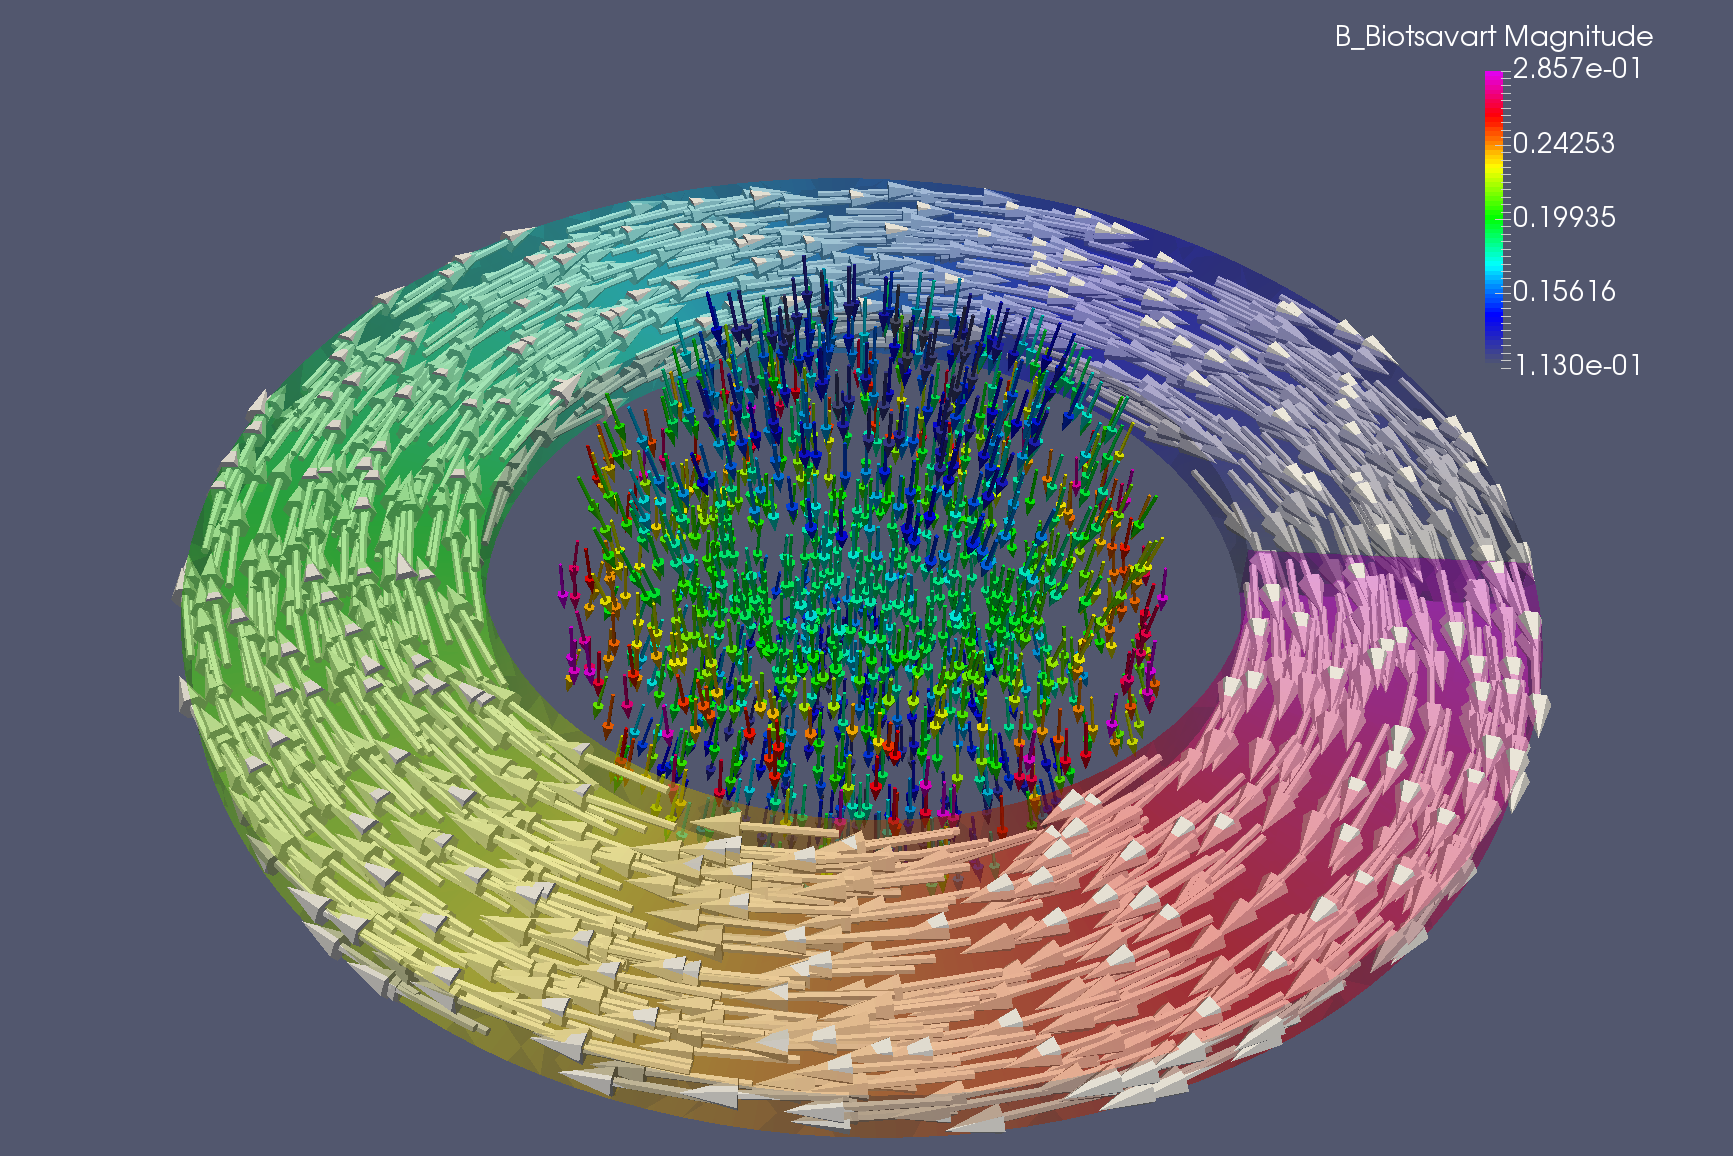
\includegraphics[width=7.0truein]{./images/learning/magnetostatic/B_and_I.png}

\centering
\end{figure}

\begin{figure}[h]{}
\centering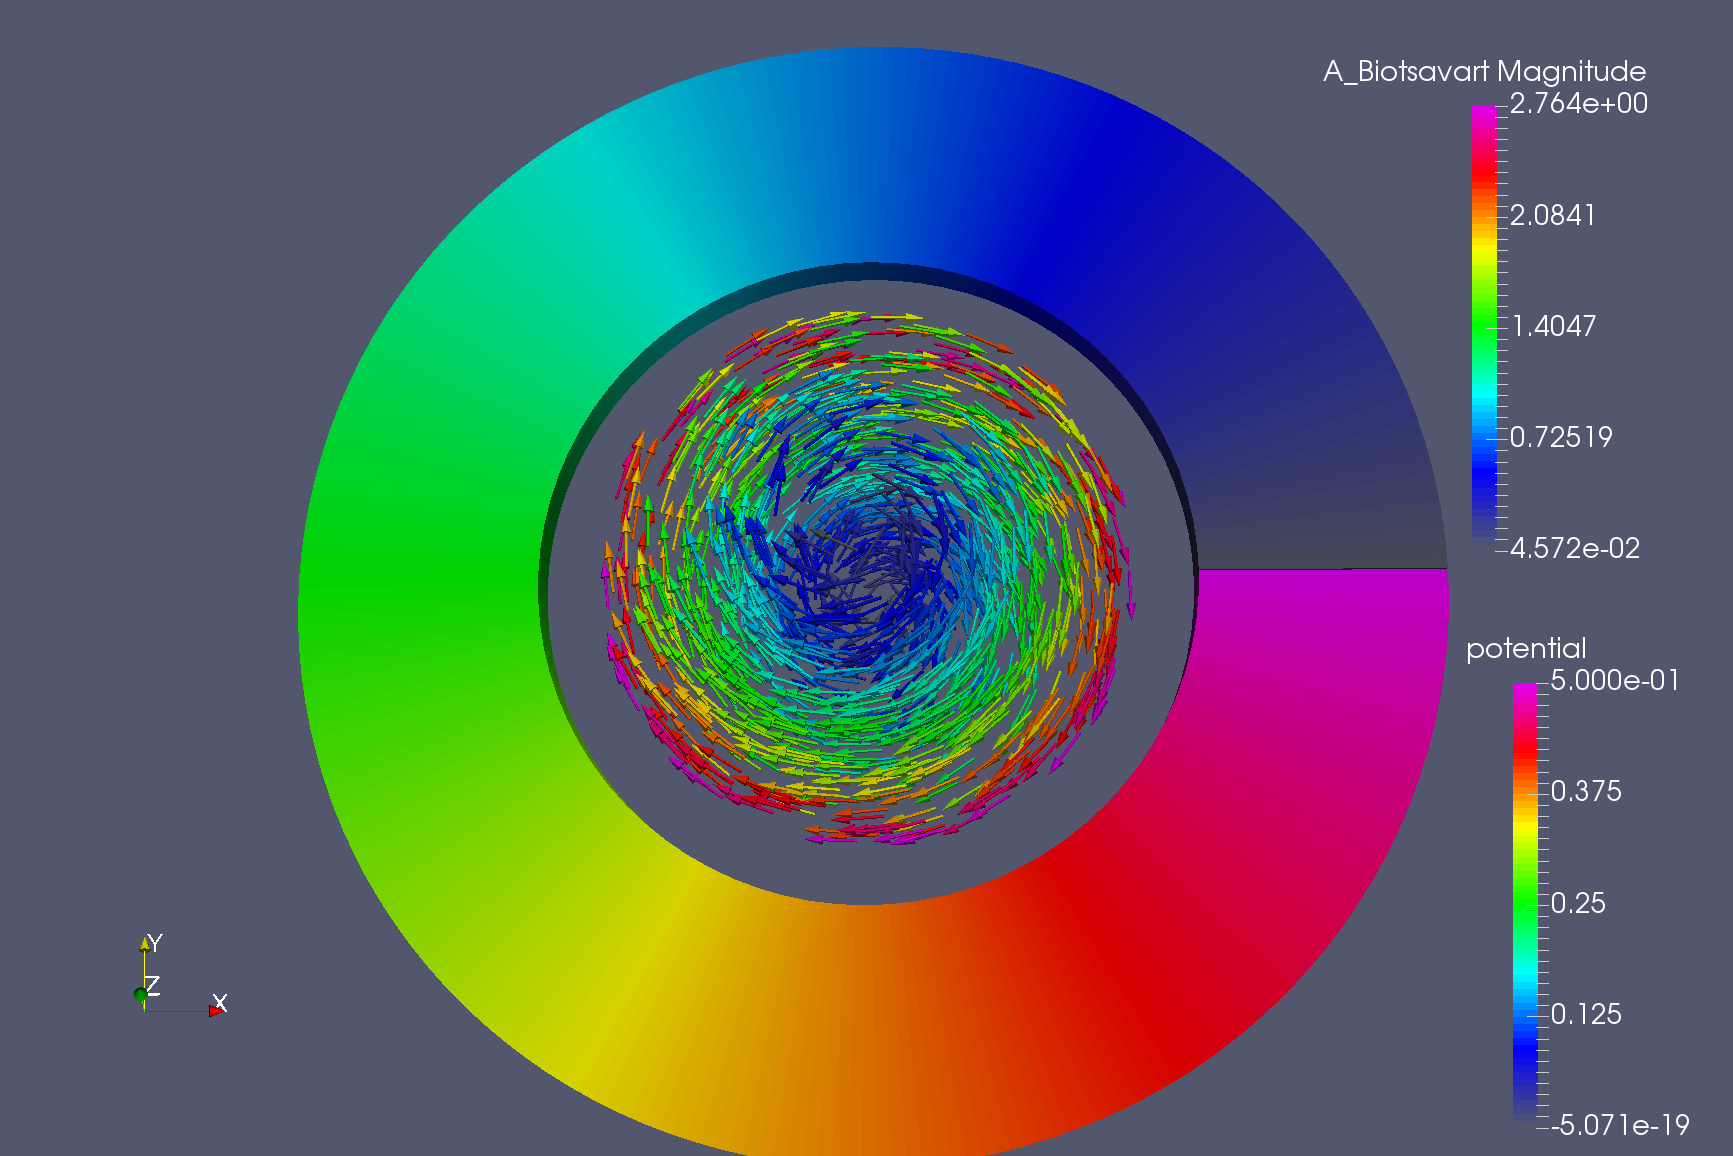
\includegraphics[width=7.0truein]{./images/learning/magnetostatic/potential_A.png}

\centering
\end{figure}

We can see that the magnetic potential (\textbf{A}) is in the same way that the current in the torus.
The scale and the direction of the magnetic field (\textbf{B}) are coherent.


\hypertarget{x-code}{\paragraph{Code}}
For the modelisation of the the torus and his box inside, we create the geometry with this file \texttt{.geo}


{\bf torus3D_box3D.geo}\vspace{-1\baselineskip}
\begin{verbatim}
// Define Main params
Unit = 1.e-3;

h=5;
r1=61.2*0.5;
r2=106.4*0.5;
L=4.61/2.;
eps=0.1;
theta1=Asin( eps/(2*r1) );
theta2=Asin( eps/(2*r2) );

// 1st quarter
Point(1) = {0, 0, -L, h};

Point(2) = {r1*Cos(theta1), eps/2., -L, h};
Point(3) = {r2*Cos(theta2), eps/2., -L, h};
Point(4) = {0, r1, -L, h};
Point(5) = {0, r2, -L, h};
Point(6) = {-r1, 0, -L, h};
Point(7) = {-r2, 0, -L, h};
Point(8) = {0, -r1, -L, h};
Point(9) = {0, -r2, -L, h};
Point(10) = {r1*Cos(-theta1), -eps/2., -L, h};
Point(11) = {r2*Cos(-theta2), -eps/2., -L, h};

Circle(1) = {2, 1, 4};
Circle(2) = {4, 1, 6};
Circle(3) = {6, 1, 8};
Circle(4) = {8, 1, 10};

Circle(5) = {3, 1, 5};
Circle(6) = {5, 1, 7};
Circle(7) = {7, 1, 9};
Circle(8) = {9, 1, 11};

Line(9) = {2, 3};
Line(10) = {10, 11};

dL=newl; Line Loop(dL) = {1:4, 10, -8, -7, -6, -5, -9};
S=news; Plane Surface(S) = {dL};

out[] = Extrude {0,0,2*L} {Surface{S};};

Physical Volume("omega") = {out[1]};
Physical Surface("top") = {out[0]};
Physical Surface("bottom") = {S};
Physical Surface("Rint") = {out[2], out[3], out[4], out[5]};
Physical Surface("Rext") = {out[7], out[8], out[9], out[10]};
Physical Surface("in") = {out[6]};
Physical Surface("out") = {out[11]};

// Define BiotSavart box
Boxdim=3;

hs=1;
np=10;

z0=-0.8*r1;
z1=-z0;

C0=newp; Point(C0) = {0, 0, 0, hs};

P0=newp; Point(P0) = {0, 0, z0, hs};
P1=newp; Point(P1) = {0, 0, z1, hs};
Q0=newp; Point(Q0) = {0, z1, 0, hs};
R0=newp; Point(R0) = {z1, 0, 0, hs};

C0P0=newl; Line(C0P0) = {C0, P0};
P0P1=newl; Line(P0P1) = {P0, P1};
BS0=newl; Circle(BS0) = {P0, C0, Q0};
BS1=newl; Circle(BS1) = {P0, C0, R0};
BS2=newl; Circle(BS2) = {Q0, C0, R0};
BS3=newl; Circle(BS3) = {Q0, C0, P1};
BS4=newl; Circle(BS4) = {R0, C0, P1};

Sb_Sph=newl; Line Loop(Sb_Sph)={BS0, BS2, -BS1};
S_Sph=newl; Ruled Surface(S_Sph)={Sb_Sph};
S2_Sph = Rotate { { 0, 0, 1 }, { 0, 0, 0 }, Pi/2. } { Duplicata{ Surface{S_Sph}; } };
S3_Sph = Rotate { { 0, 0, 1 }, { 0, 0, 0 }, 2*Pi/2. } { Duplicata{ Surface{S_Sph}; } };
S4_Sph = Rotate { { 0, 0, 1 }, { 0, 0, 0 }, 3*Pi/2. } { Duplicata{ Surface{S_Sph}; } };

Nb_Sph=newl; Line Loop(Nb_Sph)={BS2, BS4, -BS3};
N_Sph=newl; Ruled Surface(N_Sph)={Nb_Sph};
N2_Sph = Rotate { { 0, 0, 1 }, { 0, 0, 0 }, Pi/2. } { Duplicata{ Surface{N_Sph}; } };
N3_Sph = Rotate { { 0, 0, 1 }, { 0, 0, 0 }, 2*Pi/2. } { Duplicata{ Surface{N_Sph}; } };
N4_Sph = Rotate { { 0, 0, 1 }, { 0, 0, 0 }, 3*Pi/2. } { Duplicata{ Surface{N_Sph}; } };

SLoop=news; Surface Looop(SLoop)={S_Sph, N_Sph, S2_Sph, N2_Sph, S3_Sph, N3_Sph, S4_Sph, N4_Sph};
RMN=newv; Volume(RMN)={SLoop};

If ( Boxdim == 1 )
 Physical Line("box1D") = {P0P1};
EndIf

If ( Boxdim == 2 )
 Physical Surface("box2D") = {S_Sph, N_Sph, S2_Sph, N2_Sph, S3_Sph, N3_Sph, S4_Sph, N4_Sph};
EndIf

If ( Boxdim == 3 )
  Physical Volume("box3D") = {RMN};
EndIf
\end{verbatim}

the next step is to make a file \texttt{.d} which fix some parameters on the torus


{\bf torus3D.d}\vspace{-1\baselineskip}
\begin{verbatim}
#Power[MW]	Current[A]
12.5  		31000.
#Helices	N_Elem
0
#N	R1[m]  R2[m]  HalfL[m]	Rho[Ohm.m]  Alpha[1/K]	E_Max[Pa]	K[W/(m.K)]	h[W/(m^2.K)]	<T_Water>[°C]	T_Max[°C]
0.
1
# Bitter I=j1*r1*log(r2/r1)*2*L=11767.657994358965
#Type	R1	       R2	     Z1	         Z2	         J		             Rho		N_turns
1       30.6e-3    53.2e-3   -2.305e-3   2.305e-3    150833116.00212305    1         1
#1       30.6e-3    53.2e-3   -2.305e-3   2.305e-3    124827406.34658459  1         1
# Supra

#Bz(0)[tesla]	Power[MW]	Bz_total(0)[tesla]
 22.7526804266798 12.500000000 22.7526804266798

#H   B0_H[t]	Sum_B0[t] Power_H[MW]	Sum_Power[MW]



MARGE DE SECURITE CONTRAINTES= 8.0 %
\end{verbatim}

Finally we can use the \texttt{biotsavart_num} (in which we use the thermoelectric model to calculate \textbf{j}) or the \texttt{biotsavart} (in which we specify manually \textbf{j})


\begin{verbatim}
dim=3
units=mm
geofile=biotsavart_box3D.geo
geofile-path=$cfgdir
gmsh.hsize=10

conductor_volume=omega

[convergence]
max_iter=1

[functions]
j={-58.e+3*(0.5/(2*Pi))*y/(x^2+y^2),58.e+3*(0.5/(2*Pi))*x/(x^2+y^2),0}:x:y:z

[biot_savart]
conductor=omega
box=box3D

[magnetic_field-bmap]
geo-data=torus3D.d
geo-path=$cfgdir
helix-intensity=0
bitter-intensity=11767.7
supra-intensity=0
\end{verbatim}

\begin{verbatim}
dim=3
units=mm
geofile=torus3D_box3D.geo
geofile-path=$cfgdir
gmsh.hsize=10

conductor_volume=omega

[convergence]
max_iter=3

[functions]
j={58.e+3*(0.5/(2*Pi))*y/(x^2+y^2),-58.e+3*(0.5/(2*Pi))*x/(x^2+y^2),0}:x:y:z
u=0.5*atan2(y,x)/(2*Pi)*(atan2(y,x)>0)+(0.5*(atan2(y,x)+2*Pi)/(2*Pi))*(atan2(y,x)<0):x:y:z
t=362.156146169164-58.e+3/(2*0.38)*(0.5/(2*Pi))^2*log(sqrt(x*x+y*y)/39.4354779237947 )^2:x:y:z

[biot_savart]
conductor=omega
box=box3D

[magnetic_field-bmap]
geo-data=torus3D.d
geo-path=$cfgdir
helix-intensity=0
bitter-intensity=-11767.7
supra-intensity=0

[thermoelectric]
model_json=$cfgdir/biotsavart.json
weakdir=false

[electro]
pc-type=gamg
#ksp-monitor=true
ksp-rtol=1e-7
ksp-atol=1e-5
ksp-maxit=2000
ksp-use-initial-guess-nonzero=1

[thermal]
pc-type=gamg
#ksp-monitor=true
ksp-rtol=1e-8
ksp-atol=1e-6
ksp-use-initial-guess-nonzero=1
\end{verbatim}

For the numerical file, we use a \texttt{json} file like in the thermoelectric section.


\begin{verbatim}
{
    "Name": "ThermoElectric",
    "ShortName":"TE",
    "Model":"thermoelectric-linear",
    "Materials":
    {
        "omega":
        {
            "name":"copper",
            "alpha":"3.35e-3",
            "T0":"293",
            "sigma0":"58e+3",
            "k0":"0.38",
            "sigma":"sigma0/(1+alpha*(T-T0)):sigma0:alpha:T:T0",
            "k":"k0*T/((1+alpha*(T-T0))*T0):k0:T:alpha:T0"
        }
    },
    "BoundaryConditions":
    {
        "potential":
        {
            "Dirichlet":
            {
                "in":
                {
                    "expr1":"0.5",
		    "expr2":"omega"
                },
                "out":
                {
                    "expr1":"0",
		    "expr2":"omega"
                }
            }
        },
        "temperature":
        {
            "Robin":
            {
                "Rext":
                {
                    "expr1":"0.08",
                    "expr2":"293"
                },
                "Rint":
                {
                    "expr1":"0.08",
                    "expr2":"293"
                }
            }
        }
    },
    "PostProcess":
    {
        "Fields":["temperature","potential","current"]
    }
}
\end{verbatim}

\hypertarget{x-cartesian-model}{\subsection{Cartesian model}}
Until now, we only focus on the study in the center of the torus.
Indeed, the program can only calculate the magnetic potential and field outside the torus,
therefore to be able to calculate \textbf{A} and \textbf{B} around the torus that implies to create a really complex geometry.
Instead of this, we use the Cartesian model which allow to calculate \textbf{A} and \textbf{B} inside the torus,
this allow us to calculate inside the torus, then we model a large sphere to represent the air all around the conductor.


\begin{figure}[h]{}
\centering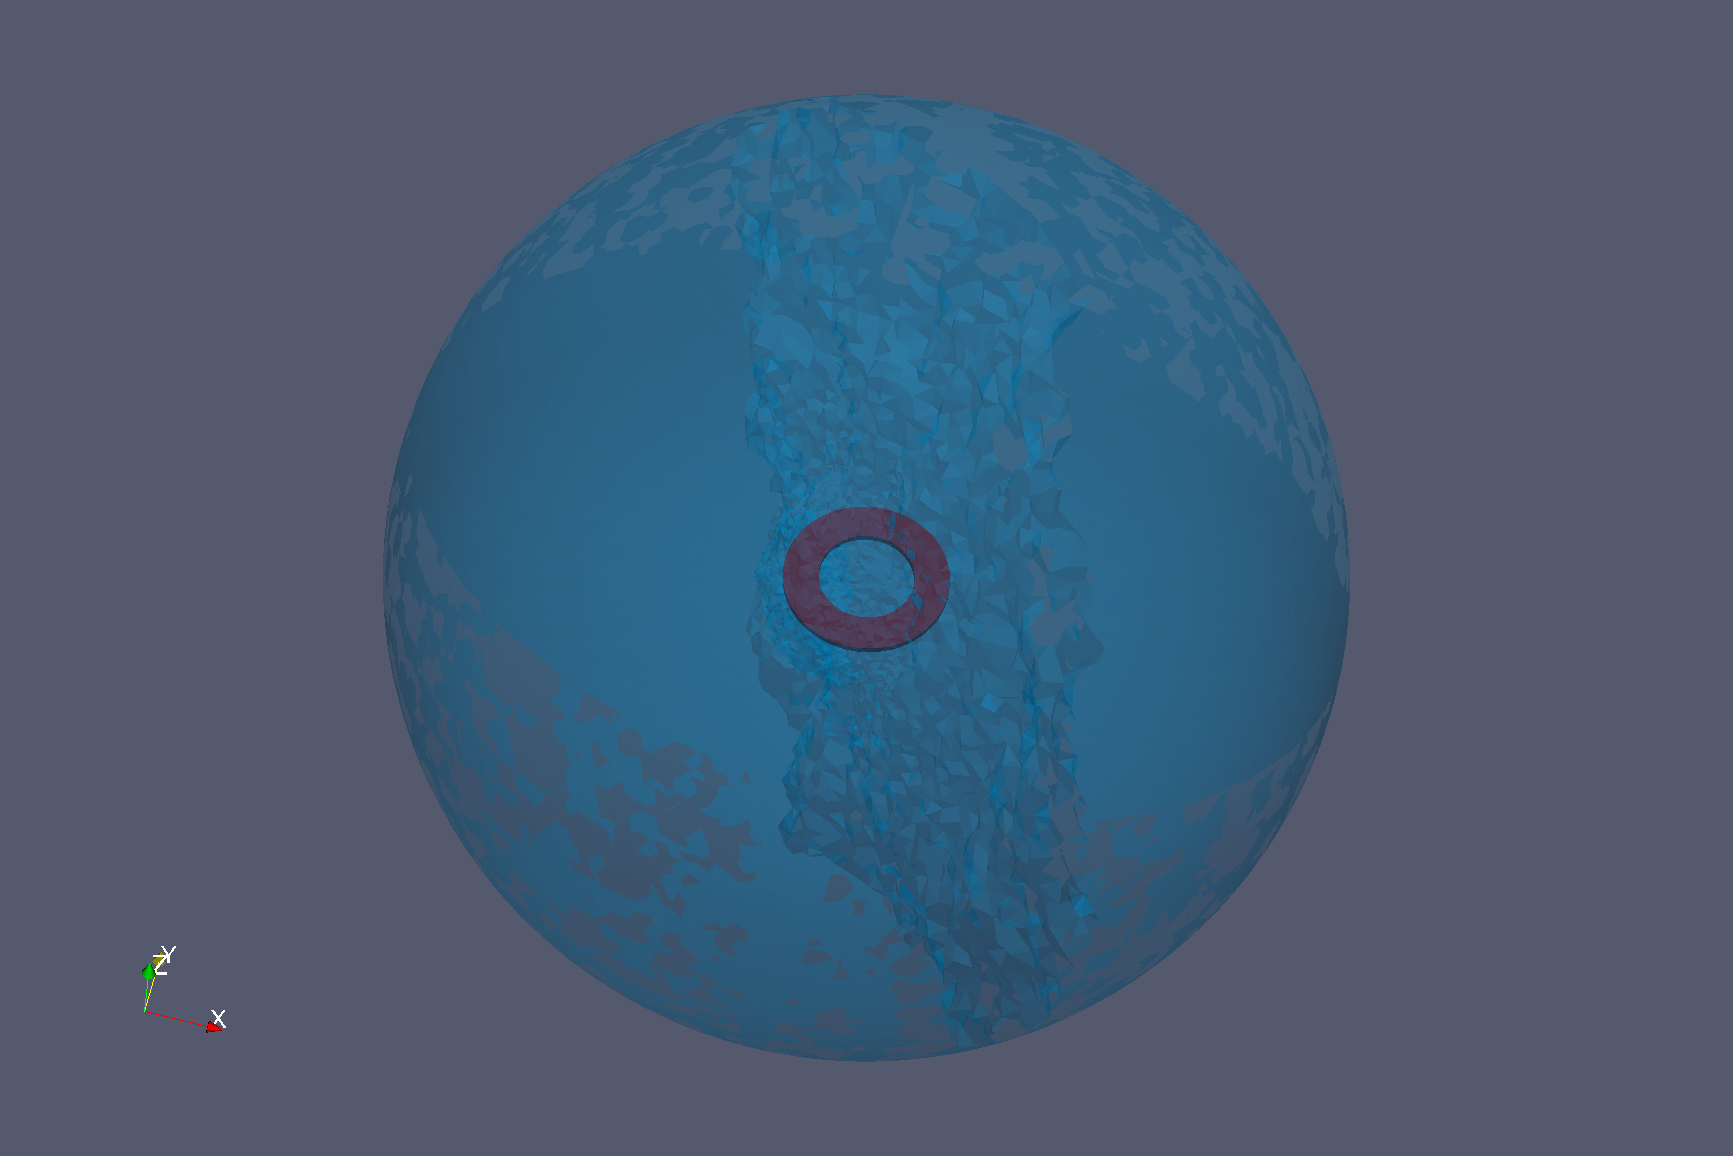
\includegraphics[width=7.0truein]{./images/learning/magnetostatic/Cartesian_model.png}
\caption{model of the torus (red) with the box (blue).}
\centering
\end{figure}

With a simple torus, we can calculate the potential analytically like before.


\begin{wrapfigure}{l}{4.75truein}
\centering\includegraphics[width=4.75truein]{./images/learning/magnetostatic/Cartesian_potential.png}


\end{wrapfigure}

\begin{wrapfigure}{r}{4.75truein}
\centering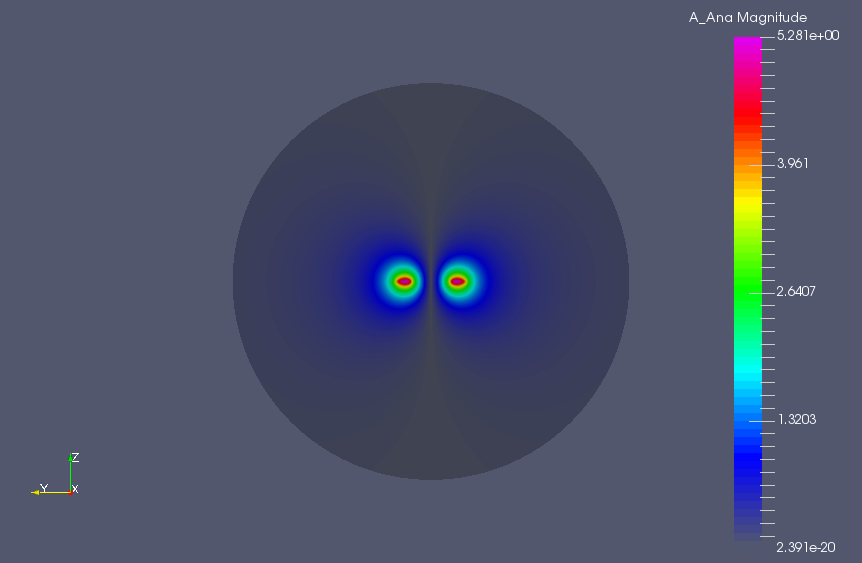
\includegraphics[width=4.75truein]{./images/learning/magnetostatic/Cartesian_potential_ana.png}


\end{wrapfigure}

Sadly, we can see that there is however some differences between the figures (on the scale)


\begin{wrapfigure}{l}{4.75truein}
\centering\includegraphics[width=4.75truein]{./images/learning/magnetostatic/Cartesian_potential_error.png}


\end{wrapfigure}

\begin{wrapfigure}{r}{4.75truein}
\centering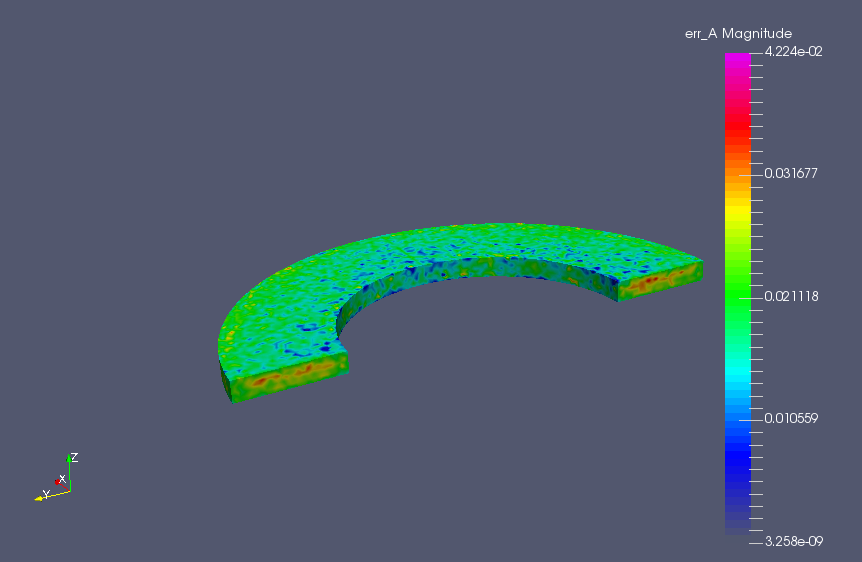
\includegraphics[width=4.75truein]{./images/learning/magnetostatic/Cartesian_potential_error_zoom.png}


\end{wrapfigure}

The maximum of the error is approximately 0.8%, located on the torus.


\hypertarget{x-\textbf{elasticity}}{\section{\textbf{Elasticity}}}
\hypertarget{x-general-presentation-of-the-files}{\subsection{General presentation of the files}}
In the continuity of the study of the magnet, we use the file already used in Thermoelectric and Magnetostatic.
We create a new file \texttt{.json} to set up the conditions for elasticity.


\begin{verbatim}
{
    "Name": "CoupledCart",
    "ShortName":"MSC",
    "Model":"Elasticity",
    "Materials":
    {
        "name_of_the_volume":
        {
            "name":"material",
            "E":"Young_modulus",
            "nu":"Poisson's_ratio",
            "alphaT":"linear_dilatation_coefficient",
            "rho":"density"
        }
    },
    "BoundaryConditions":
    {
        "condition(like displacement_x y or z)":
        {
            "type_of_condition (Dirichlet, Neumann or Robin)":
            {
                "surface_concerned":
                {
                    "expr":"_"
                },
            }
        },
        "other_condition":
        {
            ...
        },

    },
    "PostProcess":
    {
        "Fields":["displacement","Von-Mises","tresca","principal-stresses"]
    }
}
\end{verbatim}

We also need to set up the configuration file (\texttt{.cfg}) to compute the elasticity part, which consist in adding the elasticity section.


\begin{verbatim}
[elasticity]
filename=$cfgdir/quarter-torus3D-elasticity.json
on.type=elimination_symmetric
thermal_dilatation=false
do_export_all=true

# # precondtioner config
pc-type=gamg #lu,gasm,ml
ksp-monitor=true
# ksp-converged-reason=1
\end{verbatim}

\hypertarget{x-examples}{\subsection{Examples}}

\hypertarget{x-validity}{\subsection{Validity}}
\hypertarget{x-conditions}{\paragraph{Conditions}}
We consider the conductor as a solenoid with finite thickness and infinite length. This allow us to ignore the \textbf{z} components in our equations.
We admit that there is only a radial expansion.


\hypertarget{x-equations}{\paragraph{Equations}}
Taking back the equations in the \href{/math.adoc}{Maths for Hifimagnet}, we consider :



\[
div\sigma+\textbf{j}\times\textbf{b}=0
\]



With the conditions set in the previous section, we have :



\[
-\sigma_{\theta}+\frac{\partial}{\partial r}(r\sigma_{r})=-rj_{\theta}b_{z}
\]



\hypertarget{x-parameters}{\paragraph{Parameters}}
In our case (a coil of copper), we choose the parameters like this :


\begin{center}
\begin{tabular}{|c|c|c|c|c|}
\hline
$E$ & Young modulus & $[124.10^{9} ;128.10^{9}$] & $128.10^{9}$ & $Pa=kg.m^{-1} .s^{-2}$ \\ 
$\nu$ & Poisson’s ratio & 0.33 & 0.33 & - \\ 
$\alpha_{T}$ & linear dilatation coefficient & $[16,6.10^{-6} ;18.10^{-6}$] & $18.10^{-6}$ & $K^{-1}$ \\ 
$\rho$ & density & $[8920;8960$] & $8950$ & $kg.m^{-3}$ \\ 
\hline
\end{tabular}
\end{center}

\hypertarget{x-results}{\paragraph{Results}}
As we can see in this coarse mesh, the scale is coherent (he unit being in Pa).


\begin{wrapfigure}{l}{4.75truein}
\centering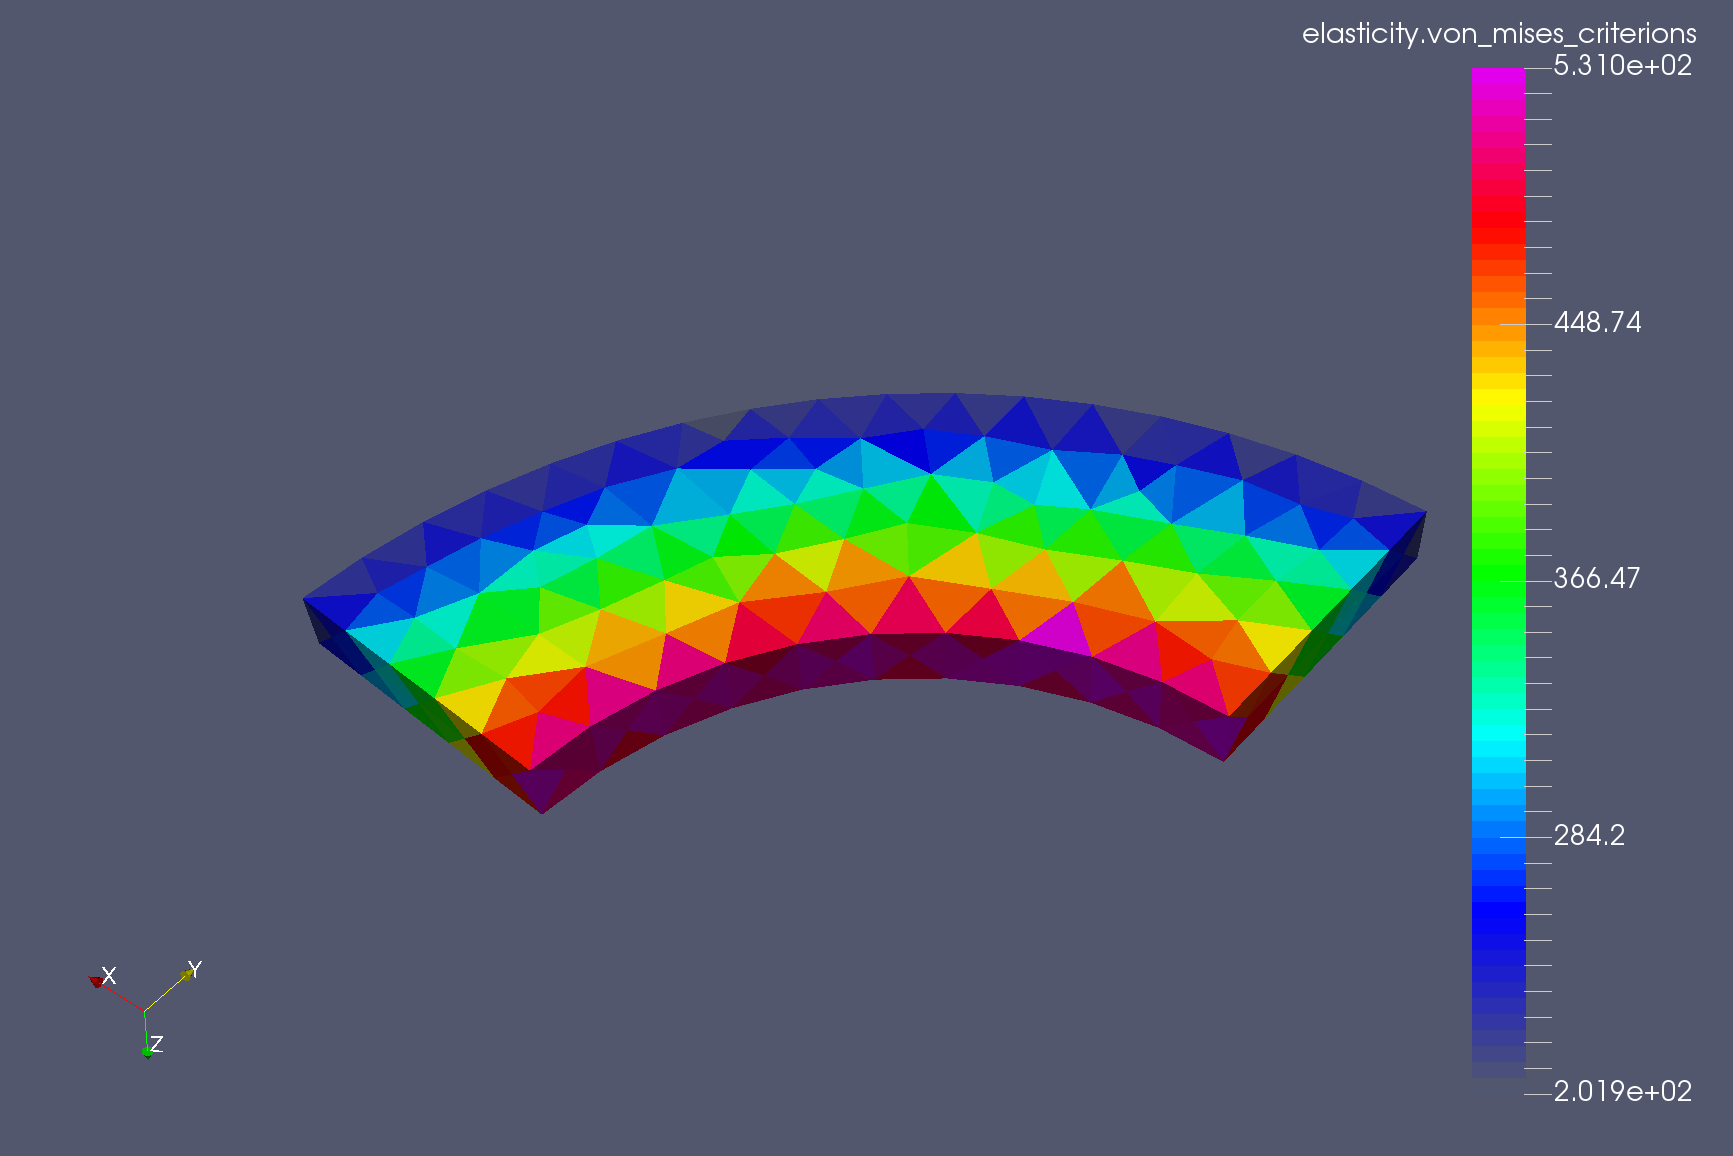
\includegraphics[width=4.75truein]{./images/learning/elasticity/Coarse_Von-Mises.png}


\end{wrapfigure}

\begin{wrapfigure}{r}{4.75truein}
\centering\includegraphics[width=4.75truein]{./images/learning/elasticity/Coarse_Tresca.png}


\end{wrapfigure}

\end{document}

